\section{Decorator-Muster}

\subsection{Problemstellung}
\begin{itemize}
\item Ein Baecker moechte verschiedene Kaffeesorten verkaufen. 
\item Es soll moeglich sein verschiedene Bonuszutaten (z.B. Sahne, Zucker, etc.) hinzuzufuegen. 
\item Hierbei kann die Menge der variieren. Es ist also moeglich sowohl eine Extra-Portion, als auch 
  zwei extra Portionen Sahne dazu zu bestellen. 
\item Ausserdem ist es moeglich verschiedene Zutaten zu kombinieren. 
\item Problem: Wenn man sich auf einfache Vererbung beschraenkt wird die Stuktur sehr schnell 
  unuebersichtlich. 
\end{itemize}

\subsection{L"osung}
Es wird zu allererst eine abstrakte Klasse Getrank gebildet, von der sowohl die Zutaten als auch 
die Kaffeesorten erben. Die Kaffesorten tun dies direkt. Sie besitzen zwei Felder fuer die 
Beschreibung und den Preis, ueber entsprechende Getter sind sie abrufbar. Nun bildet man eine 
abstrakte Wrapper-Klasse von der saemtliche Zutaten erben sollen. Jede Zutat erbt von der Wrapper 
Klasse und muessen die Getter fuer die Beschreibung / Preis neu implementieren, denn jede Zutat 
haelt eine Referenz auf ein Getraenk welches im Konstruktor gesetzt wird. Bei den Gettern wird 
die Beschreibung / Preis an die Werte des Getraenks angehaengt bzw. drauf addiert. Da alle 
Klassen von der selben Superklasse ableiten kann die Referenz nicht nur einen Kaffee ohne Zutaten 
sondern auch einen mit diesen beinhalten. Die Wrapper-Klasse ist letztendlich dazu da eine 
Schnittstelle herzustellen, damit die es sowohl geordnet ist und die Referenz wie erwaehnt 
bereits modifizierte Objekte halten kann. 

Beim Bestellen wird eine zugrunde liegende Kaffesorte gewaehlt (z.B. Espresso). Diese wird mit 
den einzelnen Zutaten "dekoriert" (Bsp. siehe main Klasse im Code). 

\subsection{Erkl"arung des Musters}
\paragraph{Definition}
Decorator - Fuegt einem Objekt dynamisch zusaetzliche Verantwortlichkeit hinzu. Dekorierer bieten 
eine flexible Alterntive zur Ableitung von Unterklassen zum Zweick der Erweiterung der 
Funktionalitaet.

\paragraph{Punkt f"ur Punkt (S.105)}
\begin{itemize}
\item Vererbung ist eine Form von Erweiterung, aber nicht notwendigerweise der beste Weg, um Ihren 
  Entwuerfen Flexiblitaet zu verleihen. 
\item Unsere Entwuerfe sollen die Erweiterung von Verhalten ermoeglichen, ohna dass dazu bestehnder 
  Code geaendert werden muesste.
\item Oft keonnen Komposition und Delegierung verwendet werden, um zur Laufzeit neue Verhalten 
  hinzuzufuegen.
\item Fuer die Erweiterung von Verhalten bietet das Decorator-Muster eine Alternative zur Ableitung 
  von Unterklassen.
\item Das Decorator-Muster schliesst einen Satz von Dekorierer-Klassen ein, die verwendet werden, um 
  konkrete Komponenten einzupacken. 
\item Dekorierer-Klassen spiegeln den Typ der Komponente wider, die sie dekorieren. (Sie haben sogar 
  tatsaechlich den gleichen Typ wie die Komponente, die sie dekorieren, entweder durch Vererbung 
  oder durch die Implementerung eines Interface.)
\item Dekorierer aendern das Verhalten der Komponenten, indem sie vor und / oder nach (oder auch an 
  Stellen von) Methodenaufrufen auf der Komponente neue Funktionalitaeten hinzufuegen. 
\item Sie koennen eine Komponente mit einer bliebigen Zahl vn Dekorierern einpacken. 
\item Dekorierer sind fuer die Clients der Komponente ueblichweise transparent, ausser wenn sich der 
  Client auf den konkreten Typ der Komponente stuetzt.
\item Dekorierer koennen in Ihren Entwuerfen zu vielen kleinen Objekten fuerhen, und eine 
  uebermaessige Verwendung kann den unuebersichtlich machen.  
\end{itemize}
 
\paragraph{Wann das Decorator-Muster ungeeignet ist}
\begin{itemize}
\item Wenn Sie mit Code arbeiten, der auf den Typ einer konkreten Komponente angewiesen ist, 
  zerbrechen Dekorierer diesen Code. Solange Sie nur Code auf Basis des abstrakten 
  Komponententyps schreiben, bleibt die Verwendung von Dekorierern fuer ihren Code transparent.
  (Muster z.B. fuer Rabatsystem beim Kaffeehaus aus diesem Kapitel ungeeignet.)
\item Dekorierer sollen den Objekten, die sie einpacken Verhalten hinzufuegen. Wenn Sie begninnen, 
  auf mehreren Schichten in der Dekoriererkette zu blicken, dann strecken Sie Decorator ueber 
  seinen eigentlichen Zweck.
\end{itemize}
  
\paragraph{Gut zu wissen}
\begin{itemize}
\item Die java.io-Klassen verwenden ebenfalls das Decorator-Muster. Es gibt diverse Streams mit 
  jeweils unterschiedlichen Aufgaben, und es gibt die Klasse FilterInputStream die als Superklasse 
  fuer verschiedene Dekorierer arbeitet.
\end{itemize}

\begin{figure}
	\centering
	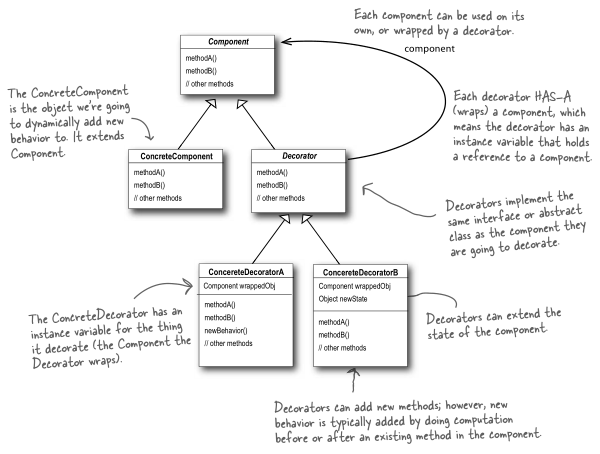
\includegraphics{decorator/img/decoratorUML}
	\caption{UML-Darstellung des Decorator-Musters}
	\label{fig:decoratorUML}
\end{figure}
